\documentclass[final]{fhnwreport}       %[mode] = draft or final
                                        %{class} = fhnwreport, article, 
                                        %          report, book, beamer, standalone
\usepackage{hyperref}
\usepackage{longtable} % To display tables on several pages


%%---Main Packages-----------------------------------------------------------------------
\usepackage[english, ngerman]{babel}	%Mul­tilin­gual sup­port for LaTeX
\usepackage[T1]{fontenc}				%Stan­dard pack­age for se­lect­ing font en­cod­ings
\usepackage[utf8]{inputenc}				%Ac­cept dif­fer­ent in­put en­cod­ings
\usepackage{lmodern}                    %The newer Font-Set
\usepackage{textcomp}					%LaTeX sup­port for the Text Com­pan­ion fonts
\usepackage{graphicx} 					%En­hanced sup­port for graph­ics
\usepackage{float}						%Im­proved in­ter­face for float­ing ob­jects
\usepackage{ifdraft}                    %Let you check if the doc is in draft mode

%%---Useful Packages---------------------------------------------------------------------
\usepackage[pdftex,dvipsnames]{xcolor}  %Driver-in­de­pen­dent color ex­ten­sions for LaTeX
\usepackage{csquotes}                   %Simpler quoting with \enquote{}
\usepackage{siunitx} 					%A com­pre­hen­sive (SI) units pack­age
\usepackage{listings}					%Type­set source code list­ings us­ing LaTeX
\usepackage[bottom]{footmisc}			%A range of foot­note op­tions
\usepackage{footnote}					%Im­prove on LaTeX's foot­note han­dling
\usepackage{verbatim}					%Reim­ple­men­ta­tion of and ex­ten­sions to LaTeX ver­ba­tim
\usepackage[textsize=footnotesize]{todonotes} %Mark­ing things to do in a LaTeX doc­u­ment

%%---Tikz Packages-----------------------------------------------------------------------
\usepackage{standalone}
\usepackage{tikz}
\usepackage{circuitikz}
\usetikzlibrary{arrows}
\usetikzlibrary{calc}
\usetikzlibrary{intersections}

%%---Math Packages-----------------------------------------------------------------------
\usepackage{amsmath}					%AMS math­e­mat­i­cal fa­cil­i­ties for LaTeX
%\usepackage{amssymb}					%Type­set­ting symbols (AMS style)
%\usepackage{array}						%Ex­tend­ing the ar­ray and tab­u­lar en­vi­ron­ments
%\usepackage{amsthm}					%Type­set­ting the­o­rems (AMS style)

%%---Table Packages----------------------------------------------------------------------
\usepackage{tabularx}					%Tab­u­lars with ad­justable-width columns
%\usepackage{longtable}
\usepackage{multirow}					%Create tab­u­lar cells span­ning mul­ti­ple rows
\usepackage{multicol}					%In­ter­mix sin­gle and mul­ti­ple columns

%%---PDF / Figure Packages---------------------------------------------------------------
\usepackage{pdfpages}					%In­clude PDF doc­u­ments in LaTeX
\usepackage{pdflscape}					%Make land­scape pages dis­play as land­scape
\usepackage{subfig}					    %Fig­ures di­vided into sub­fig­ures

%%---Other Packages----------------------------------------------------------------------
%\usepackage{xargs}                     %De­fine com­mands with many op­tional ar­gu­ments

%%---Bibliography------------------------------------------------------------------------
\usepackage[style=ieee,urldate=comp,backend=biber]{biblatex}
\addbibresource{literature/bibliography.bib}

%%---Main Settings-----------------------------------------------------------------------
\graphicspath{{./graphics/}}			%Defines the graphicspath
\geometry{twoside=false}				    %twoside=false disables the "bookstyle"
\setlength{\marginparwidth}{2cm}
\overfullrule=5em						%Creates a black rule if text goes over the margins => debugging




%%---User Definitions--------------------------------------------------------------------
%%Tabel-Definitions: (requires \usepackage{tabularx})
\newcolumntype{L}[1]{>{\raggedright\arraybackslash}p{#1}}    %column-width and alignment
\newcolumntype{C}[1]{>{\centering\arraybackslash}p{#1}}
\newcolumntype{R}[1]{>{\raggedleft\arraybackslash}p{#1}}

%%---Optional Package Settings-----------------------------------------------------------
%Listings-Settings: (requires \usepackage{listings}) => Example with Matlab Code
\lstset{language=Matlab,%
    basicstyle=\footnotesize\ttfamily,
    breaklines=false,%
    morekeywords={switch, case, otherwise},
    keywordstyle=\color{Blue},%
    tabsize=2,
    %morekeywords=[2]{1}, keywordstyle=[2]{\color{black}},
    identifierstyle=\color{Black},%
    stringstyle=\color{Purple},
    commentstyle=\color{Green},%
    showstringspaces=false,%without this there will be a symbol in the places where there is a space
    numbers=left,%
    numberstyle={\tiny \color{black}},% size of the numbers
    numbersep=9pt, % this defines how far the numbers are from the text
    %emph=[1]{word1, word2,...},emphstyle=[1]\color{red}
}										                %loads all packages, definitions and settings												
\title{Effectivenes simulation of a rebalancing
algorithm for the Lightning Network under partial
participation}          %Project Title
%\subtitle{Proposal}
\author{Proposal}          %Document Type => Technical Report, ...
\date{May 1, 2020}             %Place and Date
\begin{document}
%%---TITLEPAGE---------------------------------------------------------------------------
\selectlanguage{english}                %ngerman or english
\maketitle

\vspace*{-1cm}						    %compensates the space after the date line.
\vfill

{
\renewcommand\arraystretch{2}
\begin{center}
\begin{tabular}{>{\bf}p{4cm} l}
Organization                  &    FHNW, School of Business, Basel\\
Study program                 &    Business Information Technology\\
Author   	                  &    Tobias Koller\\
Supervisor                    &    Prof. Dr. Kaspar Riesen\\
Project sponsor               &    Prof. Dr. Thomas Hanne\\
Expert                        &    René Pickhardt
\end{tabular}
\end{center}
}
\clearpage

\pagenumbering{arabic}
\section{Introduction}

\subsection{Lightning technology}

The Lightning Network is a network that utilizes Bitcoin as its underlying system. It can therefore be described as a ``second layer'' protocol building upon the Bitcoin ``base layer''. Bitcoin is a decentralized peer-to-peer money system with no central entities. The system was designed with security and robustness being the main objectives, sacrificing other properties such as transaction throughput (speed). 

The Bitcoin system consists of nodes each maintaining a ledger of historic transactions. Each new transaction must be distributed to all nodes and validated by them. Transactions are therefore public information and must be stored by all nodes. To allow many people running a node, therefore promoting a decentralized network, the hardware requirements must be as low as possible. This is why there is a limitation of new transactions that can be made in the network causing the low transaciton throughput.

Lightning tries to solve this issue of scaling by adding a second network on top. In this network participants have payment channels open with each other. Transactions within these channels are only visible to the two channel partners but stay invisible to the rest of the network. While opening and closing a channel each requires one transaction in the base layer (Bitcoin) unlimited transactions with almost no throughput restriction can happen within the channel during its lifetime. 

It is important to note the difference between a Lightning node and a Bitcoin node. While they can run on the same system they operate in two different networks. A Bitcoin node works well individually but a Lightning node needs to have access to a Bitcoin node.

For a node to pay another node that it has no direct channel open with, he can simply route the transaction via other nodes and their channels. Since the network graph is public, the path can be chosen by the initiator of a transaction. 

A payment channel is always opened between two nodes. One of the participants acts as the initiator and provides funds for the channel in form of bitcoin. This leads to the total capacity being allocated to his balance within the channel. As soon as he starts to make payments towards the other node his balance decreases and the partners balance increases (total capacity remains constant). Transactions can only be executed if the amount is smaller than the channels capacity and if the sending node has enough local balance. Channels and their capacities are announced to the network but the distribution of balances remains private to the channel partners.

%All participant nodes maintain a full copy of the ledger which contains every transaction since the establishment of the system. To reach consensus about the actual state, nodes need to update their local copy regularly with new transactions. Those new transactions get delivered in packages, so called blocks. 

\subsection{Path finding problem}
Nodes trying to find a path in the Lightning Network work with limited information. While they know what channels are available and what their capacities are, they do not know about the balances and therefore whether the nodes can forward their payment or not. Hence, it is likely that the node attempts to make a payment which fails after because nodes had insufficient balances. The paying node needs then to find other routes and retry the payment until it succeeds. If the payment fails repeatedly it can cause unwanted delay that is bad for the user experience. 

\subsection{Starting point}
René Pickhardt's and Mariusz Nowostawski's publication ``Imbalance measure and proactive channel rebalancing algorithm for the Lightning Network'' \cite{pickhardt_imbalance_2019} serves as a base to formulate the question for this thesis. In their work they present a solution for the path finding problem in a privacy-aware payment channel network. The proposed solution includes a rebalancing protocol which the nodes of the network should follow to achieve a higher balancedness (for itself but also for the entire network). It consists of instructions to proactively rebalance their channels within their friend of a friend's network, redistributing the relative funds owned in a channel but leaving total funds owned unchanged.

Rebalancing is an activity where one node engages in a circular payment that pays himself. This is only possible when the node has at least two channels with different peers. The payment gets routed \textbf{out} through one channel and is \textbf{received back} over another channel. On the way it can use one or more hops to find back to the sender node. This procedure enables a node to change the balances of the individual channels while the total node balance stays the same. In practice there would be a fee collected by the intermediate nodes whose channels are used. In the proposed rebalancing protocol nodes would foregoe the fee and only participate in the rebalancing attempt if their balancedness improves as well.

\subsection{Problem statement}
However, these payment channel networks are decentralized by nature and no protocol change can be forced upon the node operators. Therefore, the question arises how effective this protocol change will be assuming only partial participation of nodes. What are the effects of different levels of participation on the imbalance measure \footnote{Defined as the inequality of the distribution of a nodes channel balance coefficients} of the network during repeated rebalancing cycles? What is the effect of different levels of participation on the networks ability to route payments between random nodes? 

\section{Objectives}

This section outlines the different objectives that are part of the bachelor thesis. There are mandatory objectives which must be reached and optional objectives which can be targeted if enough time is available. Although some of the simulation was already done by René Pickhardt and Mariusz Nowostawski, all the simulation code will be newly written for this thesis.

\subsection{Rebuild the Lightning Network}\label{sec:o_rebuild}

To be able to run any simulation a replicatoin of the Lightning Network must be built. This includes the extraction of node and channel information from an existing node or the acquiring of the information from other sources. 

One channel in the Lightning Network should be modeled as two directed edges between the same vertices, the network model resulting in a directed graph. This is because edge properties as balances and fees charged for routing are different in the two directions. 

One has to be aware that not all channels in the network are public. The protocol foresees the option to open private channels which are not announced to the network. This is intended for Lightning participants that do not want to participate in any routing activity but only want to send and receive. They are always start- or endpoint of a transaction and often represented by mobile wallets. Since they are not publicly known they are not part of the reconstructed network. 

\subsubsection{Optional: Develop heuristic for intial channel balances}

As the distribution of a channel's capacity is private between the two nodes there is no way to model the balances exactly. In the previous experiment the total capacity was allocated randomly to one of the two nodes. Since the channel was once funded by one of the nodes this represents an acceptable aproximation. However, it ignores the fact that many transactions might have been routed. 

A probing experiment on testnet \cite{tikhomirov_probing_2020} showed that many channels are highly unbalanced, meaning the capacity is merely on one side of the channel. An optional objective is the development of a heuristic to model the balance distribution in a way that takes into account that channels were used since they were opened.

\subsection{Reproduce simulation results from previous study}\label{sec:o_repro}
Before I can answer further questions regarding the partial participation the findings from \cite{pickhardt_imbalance_2019} must be reproduced with the constructed network. In order to do this the measurements for balancedness and improvement in routing capabilities should be transferred. Later, other measures can be introduced to compare the different levels of participation.

\subsection{Simulate different levels of participation}\label{sec:o_sim}
With objective 1 \& 2 completed we can now simulate partial participation in the new rebalancing protocol. The participation should be simulated in 10\% intervals or smaller. Af first, the participants should be determined randomly. A heuristic to chose participating nodes can be optionally introduced later.

\subsubsection{Optional: Define different balance measurement}
In the underlying research \cite{pickhardt_imbalance_2019} the measure for balance is represented by the similarity of all the channels of a node. Meaning, if all channels of a node have the same relative distribution of local to remote balance they are all equal, leading to a Gini coefficient of $0$, representing perfect balancedness. The proposed algorithm targets a smaller Gini coefficient.

Alternatively, another measure for balancedness could be defined and measured in parallel. 

\subsubsection{Optional: Define different success measurements}
The overall goal of the proactive rebalancing is to increase the networks ability to route payments. The previous work \cite{pickhardt_imbalance_2019} measures this with the success rate of random payments between all pairs of nodes along the cheapest path (based on fees) and the median possible payment size along the same paths. 

While those measures should be recorded in the different scenarios as well to provide a basis of comparison, other measures could be defined. One would be the median number of attempts to successfuly route a payment, starting from the cheapest path.

\subsubsection{Optional: Non-random selection of participants}\label{sec:selpart}
In the beginning the nodes participating in the protocol change will be selected randomly. However, this is not likely to resemble the real world as different type of node owners share characteristics that make them more or less likely to adopt the change. Nodes can be categorized by size, either total balance or number of channels, or by the centrality in the graph (closeness). These results can give insights about what participants are crucial to adopt the protocol change. 

\subsection{Analyze and visualize results}\label{sec:o_anal}

This section will define which parameters will be simulated and what measures are being recorded. Further, it shows how this data can be analyzed and what diagrams could help to visualize the results.

\subsubsection{Levels of participation}
The ratio of nodes participating in the proposed rebalancing is the most important parameter of the experiment and it represents the independent variable. In an interval of 10\% all levels (from 10\% to 100\%) should be simulated in order to get a clear picture.


Likely, the different levels of participation lead to different \textbf{average} Gini coefficients at the end of the rebalancing operation. This correlation can be shown by a line chart. When different node selection heuristics are used (see section \ref{sec:selpart}) the different heuristics can each be represented by an individual line. 

To show the distribution of the Gini coefficients in more detail a box plot with the same axes can be used.

\begin{figure}[h]
\centering
\subfloat[Shows different selection methods]{
    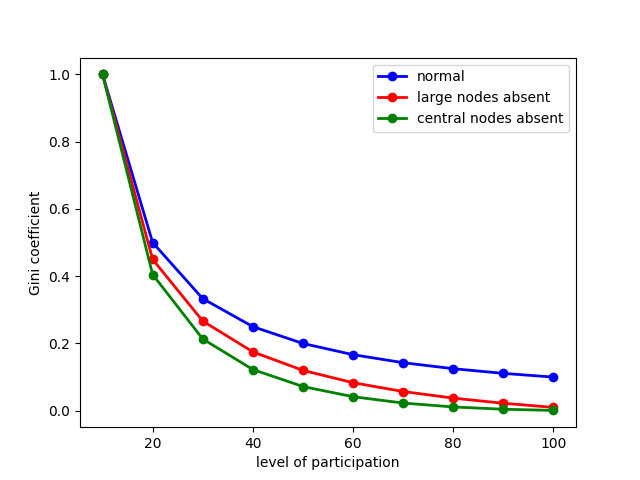
\includegraphics[width=7cm]{dummy_charts/participation.png}  
}\qquad
\subfloat[]{
    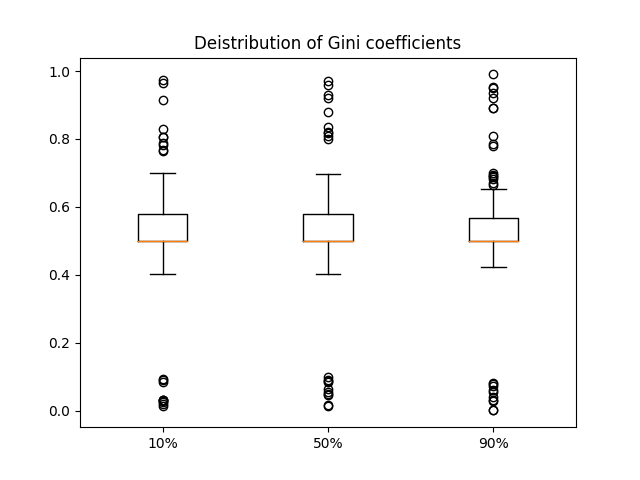
\includegraphics[width=7cm]{dummy_charts/distribution_gini.png}  
}
\caption{Ways to visualize resulting Gini coefficients.}
\label{fig:Subfigure}
\end{figure}

The x-axis can also be replaced by the number of rebalancing operations while the lines represent the different \%'s of participation. The number of data series might be reduced to avoid noise. This chart could help understand how fast a balanced network can be achieved and in what period of rebalancing the most progress is made.

\begin{figure}[h]
\centering
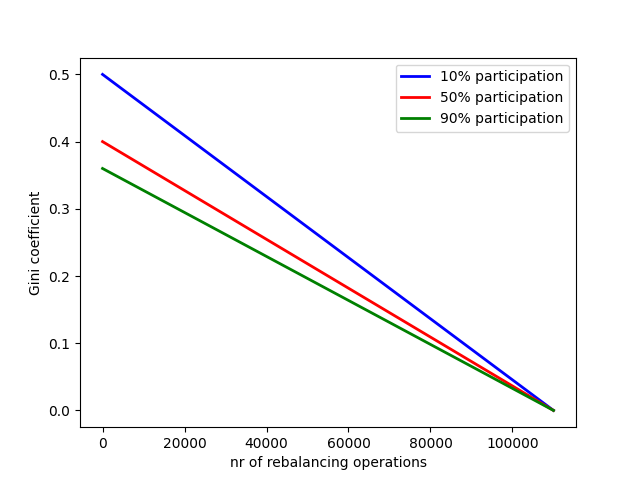
\includegraphics[width=6cm]{dummy_charts/rebal_op.png}
\caption{Development during rebalancing operations.}
\label{fig:Figure}
\end{figure}

\subsubsection{Ability to route}
The figures to measure the ability to route include ``success rate'', ``median possible payment`` and possibly ''median number of retries``. Those should be displayed in relation to the independent variable, the participation level. Again, multiple lines can be used to represent the different node selection heuristics.

\begin{figure}[h]
\centering
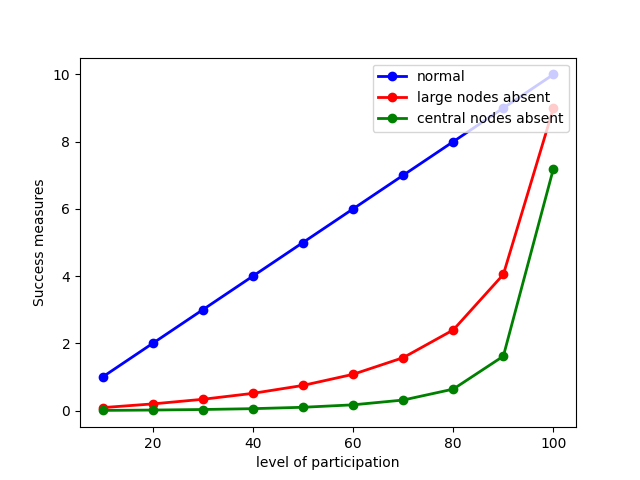
\includegraphics[width=8cm]{dummy_charts/success_measure.png}
\caption{Display different success measures}
\label{fig:Figure}
\end{figure}

To find out what percentage of cheapest paths between all nodes are able to route a certain amount of satoshis a cumulative distribution chart could be used. The x-axis displays the amount of satoshis to route and the y-axis displays the ratio of all cheapest paths that can accomodate this. Different lines represent different percentage of participation.

\begin{figure}[h]
\centering
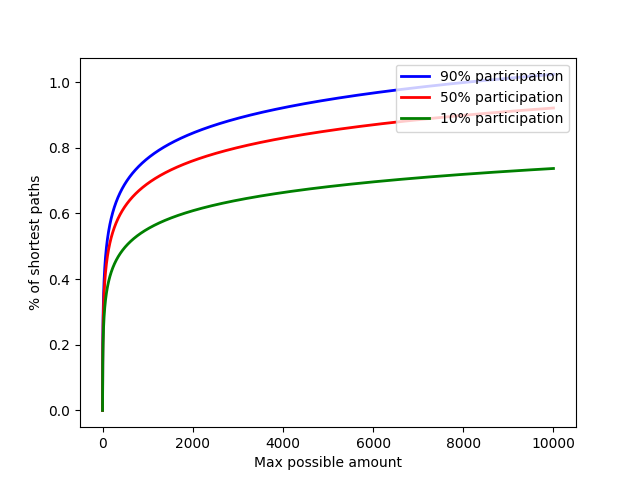
\includegraphics[width=8cm]{dummy_charts/max_payable.png}
\caption{Max payable satoshis on cheapest paths}
\label{fig:Figure}
\end{figure}

\section{Method}

In order to model the network public information from the Lithning Network is used. From a Lightning node all the channel and node information needed can be extracted.

For all further manipulations and calculations the programming language Python will be used. This includes writing code that facilitates: 
\begin{itemize}
  \item The selection of nodes, participating in the protocol change.
  \item Implement the proposed algorithm \cite[p.~3]{pickhardt_imbalance_2019}.
  \item Performing rebalancing in the network.
  \item Storing different network states for the different scenarios.
  \item Calculate different performance measures.
  \item Aggregate data.
  \item Plot graphs to visualize the results.
\end{itemize}

\section{Assumptions}
There are certain inaccuracies that need to be taken into account when the results are interpreted. 

As the network consists not only of public channels but contains also private channels it is not possible to exactly model the network. This has impact on the simulation and especially on the measured success figures. The same is true for the local balances which cannot be determined. 

The simulation only takes into account how the network changes when the nodes do rebalancing. Economic transactions that participants are performing in the real network are not simulated. They would constantly reallocate balances and undo some of the work the rebalancing algorithm is performing.

In the simulation the feasible rebalancing paths can be easily calculated as we have perfect information about all the channel balances in the network. In reality rebalancing attempts would fail often since balances not sufficient or nodes do not participate as they do not increase their balancedness.

\section{Project schedule}
The following table gives an overview of the thesis' time schedule. At the end of each week indicated the mentioned objective is planned to be achieved. The final submission deadline Friday, August 7 (midday). However, to account for unforseeable events the completion is scheduled two weeks earlier.

\renewcommand{\arraystretch}{1.5} % Default value: 1
\begin{longtable}[l]{l|p{4cm}|p{9cm}} % <-- Replaces \begin{table}, alignment must be specified here (no more tabular)  
\normalfont\textbf{Week} & \normalfont\textbf{Objective / Task} & \normalfont\textbf{Description} \\
\hline

\endfirsthead % <-- This denotes the end of the header, which will be shown on the first page only
\normalfont\textbf{Week} & \normalfont\textbf{Objective / Task} & \normalfont\textbf{Description} \\
\hline
\endhead % <-- Everything between \endfirsthead and \endhead will be shown as a header on every page

18 & Submit proposal [draft] & First version of the proposal will be submitted to René Pickhardt and Kaspar Riesen. \\
19 & Proposal approved [final] & Final version will be submitted to project sponsor for approval. \\
20 & \nameref{sec:o_rebuild} (\ref{sec:o_rebuild}) & Retrieve node and channel information and decide for an appropriate Python package to deal with networks.  \\
22 & \nameref{sec:o_repro} (\ref{sec:o_repro}) & Confirm similar results fount in previous study \cite{pickhardt_imbalance_2019} with own code and dataset. \\

25 & \nameref{sec:o_sim} (\ref{sec:o_sim}) & Write software to run the simulation. Record the described measures.  \\

27 & \nameref{sec:o_anal} (\ref{sec:o_anal}) & Aggregate the data in a way that makes them easier to present and read. Write software to plot the data in a meaningful way. Derive conclusions.  \\
29 & Submit thesis for review & Document all the steps, simulation results and findings [draft].  \\
30 & Finalize thesis & Final version ready for submission. \\

\caption{Time schedule for objectives}
\label{tab:Table1}

\end{longtable}

% \begin{table}[h]
% \renewcommand{\arraystretch}{1.3} % Default value: 1
% \begin{tabular}{L{1cm} | L{4cm} | L{9cm}}
% \normalfont\textbf{KW} & \normalfont\textbf{Objective / Task} & \normalfont\textbf{Description} \\
% \hline
% 
% 18 & Submit proposal [draft] & First version of the proposal will be submitted to René Pickhardt and Kaspar Riesen. \\
% 19 & Proposal approved [final] & Final version will be submitted to project sponsor for approval. \\
% 20 & \nameref{sec:o_rebuild} (\ref{sec:o_rebuild}) & Retrieve node and channel information and decide for an appropriate Python package to deal with networks.  \\
% 22 & \nameref{sec:o_repro} (\ref{sec:o_repro}) & Confirm similar results fount in previous study \cite{pickhardt_imbalance_2019} with own code and dataset. \\
% 
% 25 & \nameref{sec:o_sim} (\ref{sec:o_sim}) & Simulate  \\
% 
% 27 & \nameref{sec:o_anal} (\ref{sec:o_anal}) & Simulate  \\
% 29 & Submit thesis for review & kd\\
% 30 & Finalize thesis & kd \\
% \end{tabular}
% \caption{Time schedule for objectives}
% \label{tab:Table1}
% \end{table}

%%---BIBLIOGRAPHY------------------------------------------------------------------------
{\sloppypar
\printbibliography
\label{sec:lit}
}

%%---NOTES for DEBUG---------------------------------------------------------------------
\ifdraft{%Do this only if mode=draft
%%requires \usepackage{todonotes})
\newpage
\listoftodos[\section{Todo-Notes}]

\clearpage
}
{%Do this only if mode=final
}
\end{document}
